\documentclass{beamer}
\usepackage[orientation=landscape,size=custom,width=16,height=9,scale=0.5,debug]{beamerposter}

%% FONT
\usepackage[default]{comfortaa}
\usepackage[T1]{fontenc}

%% BIB
\usepackage[style=authoryear,backend=biber,url=false]{biblatex}
\addbibresource{nems.bib}

%% FIGURES
\usepackage[export]{adjustbox}
\usepackage{epstopdf}
\graphicspath{{figures/}}
\DeclareGraphicsExtensions{.pdf,.jpg}

%% FONTS
\usepackage{amsfonts,amssymb,amsmath}

%% COLORS
%\definecolor{StrongBlue}{HTML}{043C6B}
%\definecolor{SoftBlue}{HTML}{3F8FD2}
%\definecolor{StrongGreen}{HTML}{00733E}
%\definecolor{SoftGreen}{HTML}{36D88E}
%\definecolor{StrongRed}{HTML}{A64B00}
%\definecolor{SoftRed}{HTML}{FF9640}

%% RM NAV SYMBOLS
\setbeamertemplate{navigation symbols}{}

%% Content begins %%

\title{Nested Effects Models and extensions}
\subtitle{group meeting}
\date{July 15, 2016}
\author{Yuriy Sverchkov}
\institute{University of Wisconsin--Madison}

\begin{document}
\begin{frame}[plain]
  \titlepage
\end{frame}

\begin{frame}[plain]
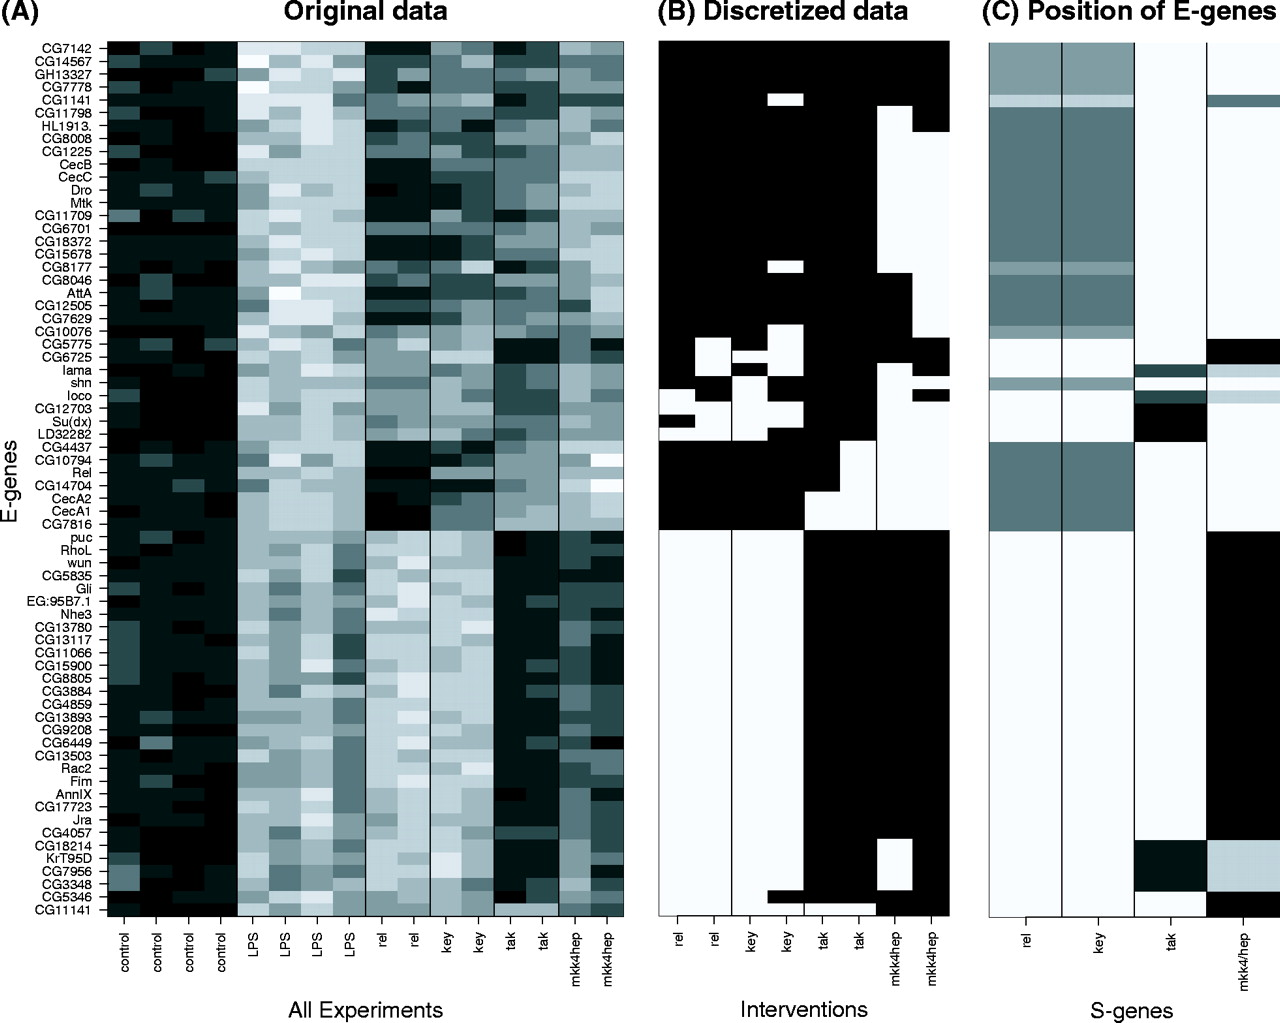
\includegraphics[valign=c,height=4cm,trim={0 0 22cm 0}, clip]{F3_large.jpg}
\hfill {\Huge $\rightarrow$} \hfill
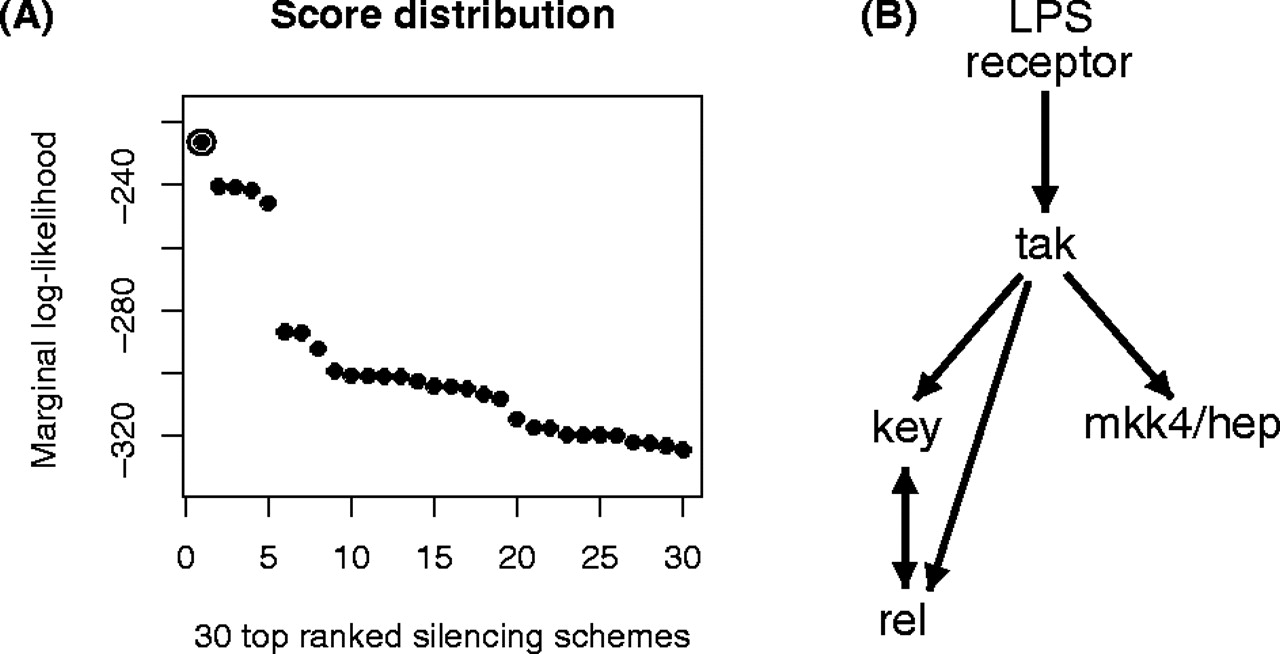
\includegraphics[valign=c,height=2cm,trim={30cm 0 0 0}, clip]{F4_large.jpg}

\scriptsize \fullcite{Markowetz01012005}
\end{frame}

\begin{frame}{Nested Effects Models (NEM)}
\begin{columns}
\column{0.4\textwidth}
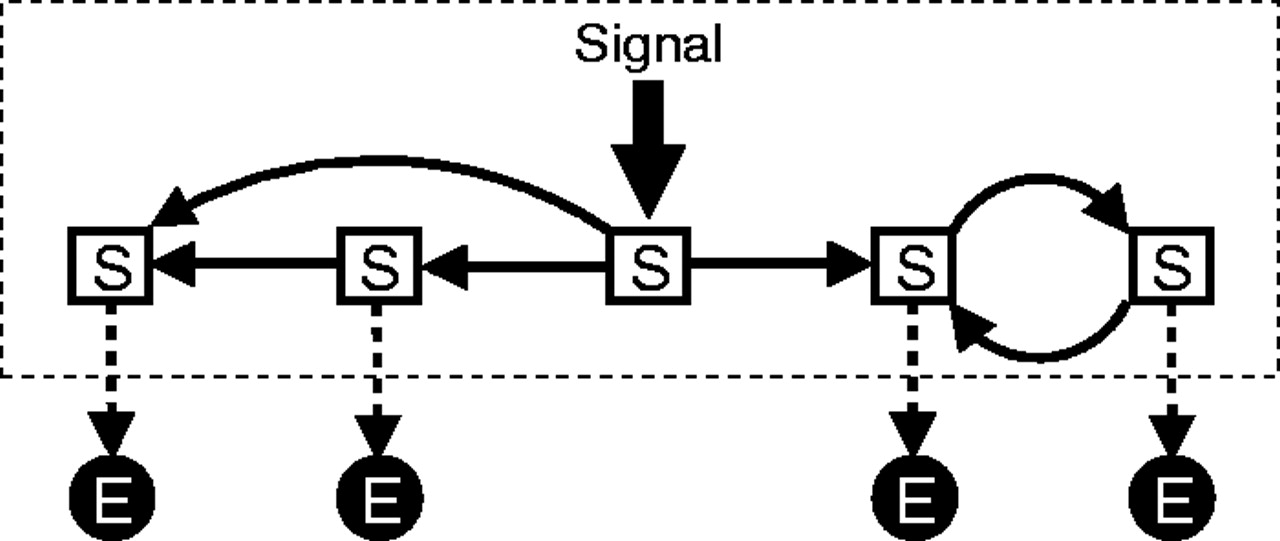
\includegraphics[width=0.9\textwidth]{F1_large.jpg}

\column{0.5\textwidth}
\begin{itemize}
  \item[S-genes] are the knockout genes
  \item[E-genes] are the measured genes
\end{itemize}
\end{columns}
\pause
\begin{itemize}
  \item \textbf{Main principle:} If an \textbf{E-gene} is differentially expressed subject to a knockout of an \textbf{S-gene}, they need to connect
  \item \textbf{Modeling constraint:} An \textbf{E-gene} can only have a direct connection to only one \textbf{S-gene}
\end{itemize}
\end{frame}

\begin{frame}{The model induces a \textbf{nesting} of E-gene sets}
\centering
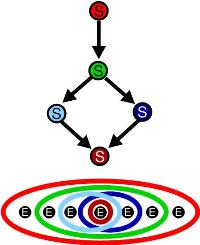
\includegraphics{NestedEffects.jpg}
\end{frame}

\end{document}